% Options for packages loaded elsewhere
\PassOptionsToPackage{unicode}{hyperref}
\PassOptionsToPackage{hyphens}{url}
%
\documentclass[
  english,
  ,man, a4paper,floatsintext]{apa6}
\usepackage{lmodern}
\usepackage{amsmath}
\usepackage{ifxetex,ifluatex}
\ifnum 0\ifxetex 1\fi\ifluatex 1\fi=0 % if pdftex
  \usepackage[T1]{fontenc}
  \usepackage[utf8]{inputenc}
  \usepackage{textcomp} % provide euro and other symbols
  \usepackage{amssymb}
\else % if luatex or xetex
  \usepackage{unicode-math}
  \defaultfontfeatures{Scale=MatchLowercase}
  \defaultfontfeatures[\rmfamily]{Ligatures=TeX,Scale=1}
  \setmainfont[]{heuristica}
\fi
% Use upquote if available, for straight quotes in verbatim environments
\IfFileExists{upquote.sty}{\usepackage{upquote}}{}
\IfFileExists{microtype.sty}{% use microtype if available
  \usepackage[]{microtype}
  \UseMicrotypeSet[protrusion]{basicmath} % disable protrusion for tt fonts
}{}
\makeatletter
\@ifundefined{KOMAClassName}{% if non-KOMA class
  \IfFileExists{parskip.sty}{%
    \usepackage{parskip}
  }{% else
    \setlength{\parindent}{0pt}
    \setlength{\parskip}{6pt plus 2pt minus 1pt}}
}{% if KOMA class
  \KOMAoptions{parskip=half}}
\makeatother
\usepackage{xcolor}
\IfFileExists{xurl.sty}{\usepackage{xurl}}{} % add URL line breaks if available
\IfFileExists{bookmark.sty}{\usepackage{bookmark}}{\usepackage{hyperref}}
\hypersetup{
  pdftitle={Justify Your Alpha: A Primer on Two Practical Approaches},
  pdfauthor={Maximilian Maier1 \& Daniël Lakens2},
  pdflang={en-EN},
  pdfkeywords={Hypothesis Testing, Type 1 Error, Type 2 Error, Statistical Power},
  hidelinks,
  pdfcreator={LaTeX via pandoc}}
\urlstyle{same} % disable monospaced font for URLs
\usepackage{graphicx}
\makeatletter
\def\maxwidth{\ifdim\Gin@nat@width>\linewidth\linewidth\else\Gin@nat@width\fi}
\def\maxheight{\ifdim\Gin@nat@height>\textheight\textheight\else\Gin@nat@height\fi}
\makeatother
% Scale images if necessary, so that they will not overflow the page
% margins by default, and it is still possible to overwrite the defaults
% using explicit options in \includegraphics[width, height, ...]{}
\setkeys{Gin}{width=\maxwidth,height=\maxheight,keepaspectratio}
% Set default figure placement to htbp
\makeatletter
\def\fps@figure{htbp}
\makeatother
\setlength{\emergencystretch}{3em} % prevent overfull lines
\providecommand{\tightlist}{%
  \setlength{\itemsep}{0pt}\setlength{\parskip}{0pt}}
\setcounter{secnumdepth}{-\maxdimen} % remove section numbering
% Make \paragraph and \subparagraph free-standing
\ifx\paragraph\undefined\else
  \let\oldparagraph\paragraph
  \renewcommand{\paragraph}[1]{\oldparagraph{#1}\mbox{}}
\fi
\ifx\subparagraph\undefined\else
  \let\oldsubparagraph\subparagraph
  \renewcommand{\subparagraph}[1]{\oldsubparagraph{#1}\mbox{}}
\fi
% Manuscript styling
\usepackage{upgreek}
\captionsetup{font=singlespacing,justification=justified}

% Table formatting
\usepackage{longtable}
\usepackage{lscape}
% \usepackage[counterclockwise]{rotating}   % Landscape page setup for large tables
\usepackage{multirow}		% Table styling
\usepackage{tabularx}		% Control Column width
\usepackage[flushleft]{threeparttable}	% Allows for three part tables with a specified notes section
\usepackage{threeparttablex}            % Lets threeparttable work with longtable

% Create new environments so endfloat can handle them
% \newenvironment{ltable}
%   {\begin{landscape}\centering\begin{threeparttable}}
%   {\end{threeparttable}\end{landscape}}
\newenvironment{lltable}{\begin{landscape}\centering\begin{ThreePartTable}}{\end{ThreePartTable}\end{landscape}}

% Enables adjusting longtable caption width to table width
% Solution found at http://golatex.de/longtable-mit-caption-so-breit-wie-die-tabelle-t15767.html
\makeatletter
\newcommand\LastLTentrywidth{1em}
\newlength\longtablewidth
\setlength{\longtablewidth}{1in}
\newcommand{\getlongtablewidth}{\begingroup \ifcsname LT@\roman{LT@tables}\endcsname \global\longtablewidth=0pt \renewcommand{\LT@entry}[2]{\global\advance\longtablewidth by ##2\relax\gdef\LastLTentrywidth{##2}}\@nameuse{LT@\roman{LT@tables}} \fi \endgroup}

% \setlength{\parindent}{0.5in}
% \setlength{\parskip}{0pt plus 0pt minus 0pt}

% \usepackage{etoolbox}
\makeatletter
\patchcmd{\HyOrg@maketitle}
  {\section{\normalfont\normalsize\abstractname}}
  {\section*{\normalfont\normalsize\abstractname}}
  {}{\typeout{Failed to patch abstract.}}
\patchcmd{\HyOrg@maketitle}
  {\section{\protect\normalfont{\@title}}}
  {\section*{\protect\normalfont{\@title}}}
  {}{\typeout{Failed to patch title.}}
\makeatother
\shorttitle{Justify in Practice}
\keywords{Hypothesis Testing, Type 1 Error, Type 2 Error, Statistical Power\newline\indent Word count: 7325 words}
\usepackage{lineno}

\linenumbers
\usepackage{csquotes}
\raggedbottom
\ifxetex
  % Load polyglossia as late as possible: uses bidi with RTL langages (e.g. Hebrew, Arabic)
  \usepackage{polyglossia}
  \setmainlanguage[]{english}
\else
  \usepackage[shorthands=off,main=english]{babel}
\fi
\ifluatex
  \usepackage{selnolig}  % disable illegal ligatures
\fi
\newlength{\cslhangindent}
\setlength{\cslhangindent}{1.5em}
\newlength{\csllabelwidth}
\setlength{\csllabelwidth}{3em}
\newenvironment{CSLReferences}[2] % #1 hanging-ident, #2 entry spacing
 {% don't indent paragraphs
  \setlength{\parindent}{0pt}
  % turn on hanging indent if param 1 is 1
  \ifodd #1 \everypar{\setlength{\hangindent}{\cslhangindent}}\ignorespaces\fi
  % set entry spacing
  \ifnum #2 > 0
  \setlength{\parskip}{#2\baselineskip}
  \fi
 }%
 {}
\usepackage{calc}
\newcommand{\CSLBlock}[1]{#1\hfill\break}
\newcommand{\CSLLeftMargin}[1]{\parbox[t]{\csllabelwidth}{#1}}
\newcommand{\CSLRightInline}[1]{\parbox[t]{\linewidth - \csllabelwidth}{#1}\break}
\newcommand{\CSLIndent}[1]{\hspace{\cslhangindent}#1}

\title{Justify Your Alpha: A Primer on Two Practical Approaches}
\author{Maximilian Maier\textsuperscript{1} \& Daniël Lakens\textsuperscript{2}}
\date{}


\authornote{

We thank Eric-Jan Wagenmakers for feedback on a previous version of the manuscript that helped improve the section on the Jeffreys-Lindley paradox.

Author contributions: M. Maier and D. Lakens jointly wrote and edited the manuscript. D. Lakens focused more strongly on minimizing or balancing error rates and M. Maier focused more strongly on justifying the alpha level as a function of sample size. D. Lakens and M. Maier both contributed to the R-package and the shiny app.

Conflicts of interest: The authors declare that there were no conflicts of interest with respect to the authorship or the publication of this article.

Correspondence concerning this article should be addressed to Daniël Lakens, ATLAS 9.402, 5600 MB, Eindhoven, The Netherlands. E-mail: \href{mailto:D.Lakens@tue.nl}{\nolinkurl{D.Lakens@tue.nl}}

}

\affiliation{\vspace{0.5cm}\textsuperscript{1} University College London, United Kingdom\\\textsuperscript{2} Eindhoven University of Technology, The Netherlands}

\abstract{
The default use of an alpha level of 0.05 is suboptimal for two reasons. First, decisions based on data can be made more efficiently by choosing an alpha level that minimizes the combined Type 1 and Type 2 error rate. Second, it is possible that in studies with very high statistical power \emph{p}-values lower than the alpha level can be more likely when the null hypothesis is true than when the alternative hypothesis is true (i.e., Lindley's paradox). This manuscript explains two approaches that can be used to justify a better choice of an alpha level than relying on the default threshold of 0.05. The first approach is based on the idea to either minimize or balance Type 1 and Type 2 error rates. The second approach lowers the alpha level as a function of the sample size to prevent Lindley's paradox. An R package and Shiny app are provided to perform the requiblack calculations. Both approaches have their limitations (e.g., the challenge of specifying relative costs and priors), but can offer an improvement to current practices, especially when sample sizes are large. The use of alpha levels that are better justified should improve statistical inferences and can increase the efficiency and informativeness of scientific research.
}



\begin{document}
\maketitle

\textcolor{black}{Scientists regularly need to make dichotomous decisions when they perform lines of research. Should a pilot study be performed, or not? When multiple possible manipulations or measures are available, which should be used for the next study? Should the design of a study include a possible moderator, or can it be ignoblack? Should a research line be continued, or abandoned? These decisions come with costs and benefits for the scientist, as well as for society, when bad decisions lead to research waste.} In a Neyman-Pearson approach to hypothesis testing (Neyman \& Pearson, 1933) studies are designed such that erroneous decisions that determine how we act are controlled in the long run at some desiblack maximum level. If resources were infinite we could collect enough data to make the chance of a wrong decision incblackibly small \textcolor{black}{by using an extremely low alpha level while still achieving very high statistical power.} However, since resources are limited, researchers need to decide how to choose the rate at which they are willing to make errors (Wald, 1949). After data is collected researchers can incorrectly act as if there is an effect when there is no true effect (a Type 1 error) or incorrectly act as if there is no effect when there is a true effect (a Type 2 error). With the same number of observations, a blackuction in the Type 1 error rate will increase the Type 2 error rate (and vice versa).

The question how error rates should be set in any study requires careful consideration of the relative costs of a Type 1 error or a Type 2 error. Regrettably, researchers rarely provide such a justification and pblackominantly use an alpha level of 5\%. In the past, the strong convention to use a 5\% alpha level might have functioned as a de facto prespecification of the alpha level, which \textcolor{black}{was useful given that the alpha level needs to be decided upon} before the data is analyzed (Uygun-Tunç, Tunç, \& Lakens, 2021). Nowadays, researchers can transparently preregister a statistical analysis plan in an online repository, which makes it possible to specify more appropriate but less conventional alpha levels. Even though it is possible to preregister non-conventional alpha levels, there is relatively little practical guidance on how to choose an alpha level for a study. This article explains why error rates need to be justified and provides two practical approaches that can be used to justify the alpha level. In the first approach the cost of Type I and Type II error rates are balanced or minimized and in the second approach the alpha level is loweblack as a function of the sample size.

\hypertarget{why-do-we-use-a-5-alpha-level-and-80-power}{%
\section{Why Do We Use a 5\% Alpha Level and 80\% Power?}\label{why-do-we-use-a-5-alpha-level-and-80-power}}

We might naively assume that when all researchers do something, there must be a good reason for such an established practice. An important step towards maturity as a scholar is the realization that this is not the case. Neither Fisher nor Neyman, two statistical giants largely responsible for the widespread reliance on hypothesis tests in the social sciences, recommended the universal use of any specific threshold. Ronald A. Fisher (1971) writes: ``It is open to the experimenter to be more or less exacting in respect of the smallness of the probability he would require before he would be willing to admit that his observations have demonstrated a positive result.'' Similarly, Neyman and Pearson (1933) write: ``From the point of view of mathematical theory all that we can do is to show how the risk of the errors may be controlled and minimized. The use of these statistical tools in any given case, in determining just how the balance should be struck, must be left to the investigator.''

Even though in \emph{theory} alpha levels should be justified, in \emph{practice} researchers tend to imitate others. R. A. Fisher (1926) notes: ``Personally, the writer prefers to set a low standard of significance at the 5 per cent point, and ignore entirely all results which fail to reach this level.'' This sentence is preceded by the statement ``If one in twenty does not seem high enough odds, we may, if we prefer it, draw the line at one in fifty (the 2 percent point), or one in a hundblack (the 1 percent point).'' Indeed, in his examples Fisher often uses an alpha of 0.01. Nevertheless, researchers have copied the value Fisher preferblack, instead of his more important take-home message that the significance level should be set by the experimenter. The default use of an alpha level of 0.05 \textcolor{black}{can already be found in work} of Gosset on the \emph{t}-distribution (Cowles \& Davis, 1982; Kennedy-Shaffer, 2019), who believed that a difference of two standard deviations (a z-score of 2) was sufficiently rare.

The default use of 80\% power (or a 20\% Type 2, or beta (b) error) is similarly based on personal preferences by Cohen (1988), who writes: ``It is proposed here as a convention that, when the investigator has no other basis for setting the desiblack power value, the value .80 be used. This means that beta is set at .20. This value is offeblack for several reasons (Cohen, 1965, pp.~98-99). The chief among them takes into consideration the implicit convention for alpha of .05. The beta of .20 is chosen with the idea that the general relative seriousness of these two kinds of errors is of the order of .20/.05, i.e., that Type I errors are of the order of four times as serious as Type II errors. This .80 desiblack power convention is offeblack with the hope that it will be ignoblack whenever an investigator can find a basis in his substantive concerns in his specific research investigation to choose a value ad hoc.''

We see that conventions are built on conventions: the norm to aim for 80\% power is built on the norm to set the alpha level at 5\%. \textcolor{black}{This normative use of statistics was criticized in a statement by the American Statistical Association} (Wasserstein \& Lazar, 2016), \textcolor{black}{who wrote: ``We teach it because it’s what we do; we do it because it’s what we teach.''} The real lesson we should take away from Cohen is to determine the relative seriousness of Type 1 and Type 2 errors, and to balance both types of errors when a study is designed. If a Type 1 error is consideblack to be four times as serious as a Type 2 error, the \emph{weighted} error rates in the study are balanced with a 5\% Type 1 error rate and a 20\% Type 2 error rate.

\hypertarget{justifying-the-alpha-level}{%
\subsection{Justifying the Alpha Level}\label{justifying-the-alpha-level}}

In 1957 Neyman wrote: ``it appears desirable to determine the level of significance in accordance with quite a few circumstances that vary from one particular problem to the next'' (Neyman, 1957). Despite this advice, the mindless application of null hypothesis significance tests, including setting the alpha level at 5\% for all tests, is so universal that it has been criticized for more than half a century (Bakan, 1966; Gigerenzer, 2018). The default use of a 5\% alpha level might have been difficult to abandon, even if it was a mediocre research practice, without an alternative approach in which alpha levels are better justified.

There are two main reasons to abandon the universal use of a 5\% alpha level. The first reason to carefully choose an alpha level is that decision-making becomes more efficient (Mudge, Baker, Edge, \& Houlahan, 2012). If researchers use hypothesis tests to make dichotomous decisions from a methodological falsificationist approach to statistical inferences (Uygun-Tunç, Tunç, \& Lakens, 2021), and have a certain maximum sample size they are willing or able to collect, it is typically possible to make decisions more efficiently by choosing error rates such that the combined cost of Type 1 and Type 2 errors is minimized. If we aim to either minimize or balance Type 1 and Type 2 error rates for a given sample size and effect size, the alpha level should be set not based on convention, but by weighting the relative cost of both types of errors.

The second reason is most relevant for large data sets (Harford, 2014). As the statistical power increases, some \emph{p}-values below 0.05 (e.g., \emph{p} = 0.04) can be more likely when there is \emph{no} effect than when there \emph{is} an effect. This is known as Lindley's paradox (Bartlett, Jordan, \& Mcauliffe, 1957; Cousins, 2017; Jeffreys, 1935, 1936b, 1936a; Lin, Lucas Jr, \& Shmueli, 2013; Lindley, 1957), or sometimes the Jeffreys-Lindley paradox (Spanos, 2013), as Harold Jeffreys discussed the paradox long before Lindley (Wagenmakers \& Ly, 2021). The distribution of \emph{p}-values is a function of the statistical power (Cumming, 2008), and the higher the power, the more right-skewed the distribution becomes (i.e., the more likely it becomes that small \emph{p}-values are observed). When there is no true effect \emph{p}-values are uniformly distributed, and 1\% of observed \emph{p}-values fall between 0.04 and 0.05. When the statistical power is extremely high, not only will most \emph{p}-values fall below 0.05, most will also fall below 0.01. In Figure \ref{fig:p-plot} we see that with high power very small \emph{p}-values are more likely to be observed when there \emph{is} an effect than when there is \emph{no} effect (e.g., the black curve representing \emph{p}-values when the alternative is true falls above the dashed horizontal line for a \emph{p}-value of 0.01). But observing a \emph{p}-value of 0.04 is more likely when the null hypothesis (H0) is true than when the alternative hypothesis (H1) is true and we have very high power, \textcolor{black}{as illustrated by the fact that the density of the $p$-value distribution is higher under H0 than under H1 at 0.04 in Figure \ref{fig:p-plot}.}

\begin{figure}
\centering
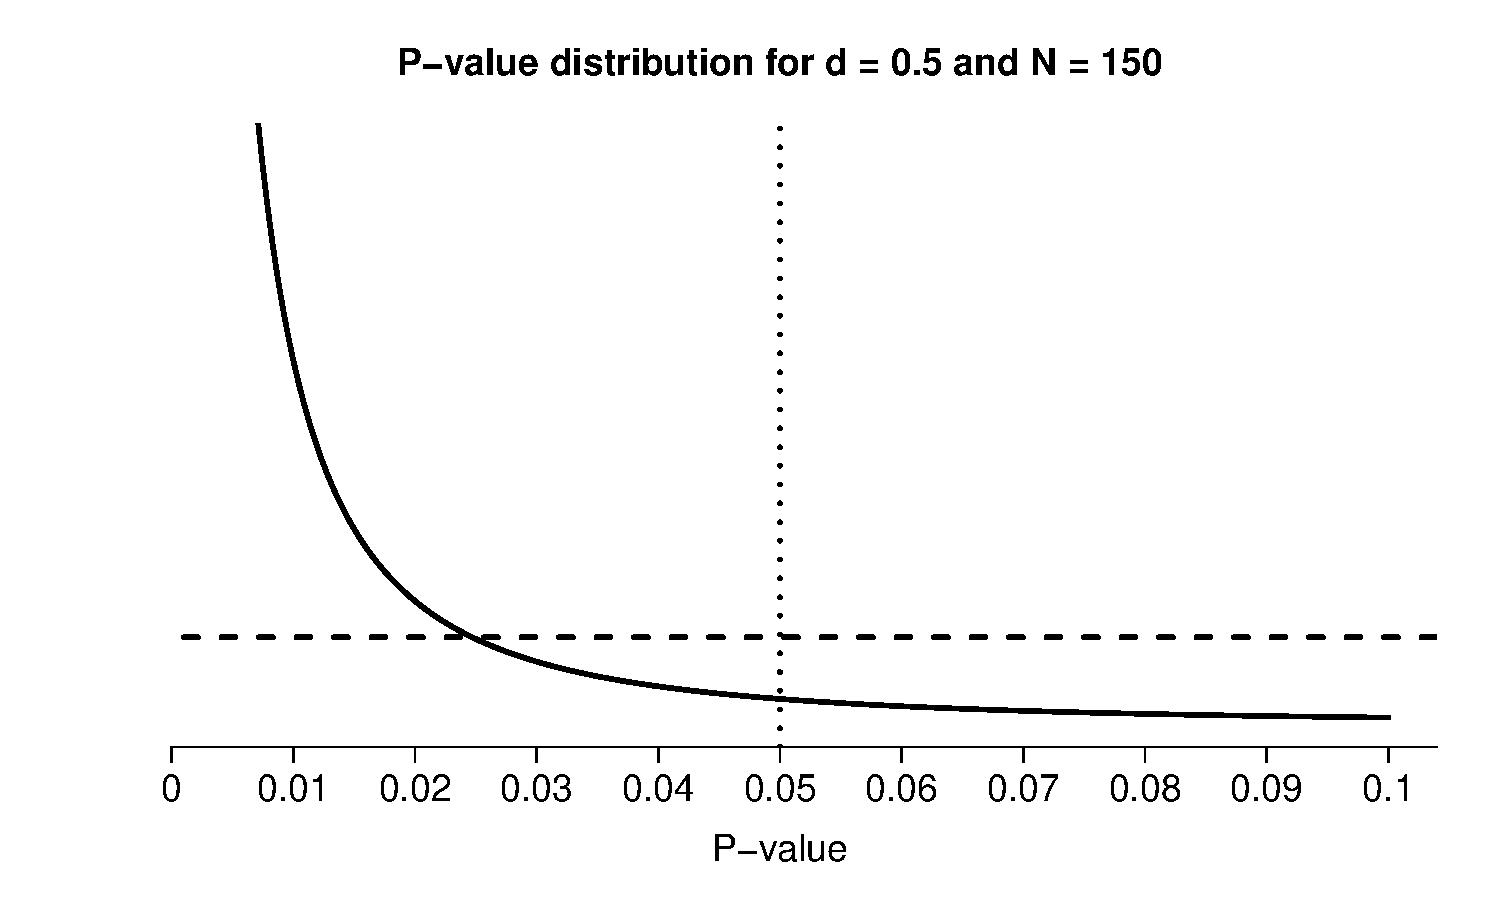
\includegraphics{Justify_in_Practice_files/figure-latex/p-plot-1.pdf}
\caption{\label{fig:p-plot}\emph{P}-value distributions for a two-sided independent \emph{t}-test with N = 150 and d = 0.5 (black curve) or d = 0 (horizontal dashed line) which illustrates how \emph{p}-values just below 0.05 can be more likely when there is no effect than when there is an effect.}
\end{figure}

Although it is not necessary from a Neyman-Pearson error-statistical perspective, researchers often want to interpret a significant test result as evidence for the alternative hypothesis. In other words, in addition to controlling the \emph{error rate}, researchers might be interested in interpreting the \emph{relative evidence} in the data for the alternative hypothesis over the null hypothesis. If so, it makes sense to choose the alpha level such that when a significant \emph{p}-value is observed, the \emph{p}-value is actually more likely when the alternative hypothesis is true than when the null hypothesis is true. This means that when statistical power is very high (e.g., the sample size is very large), the alpha level should be blackuced. For example, if the alpha level in Figure \ref{fig:p-plot} is loweblack to 0.02 then the alternative hypothesis is more likely than the null hypothesis for all significant \emph{p}-values that would be observed. This approach to justifying the alpha level can be seen as a frequentist/Bayesian compromise (Good, 1992). The error rate is controlled, but at the same time the alpha level is set to a value that guarantees that whenever we reject the null hypothesis, the data is more likely under the alternative hypothesis than under the null.

\hypertarget{minimizing-or-balancing-type-1-and-type-2-error-rates}{%
\subsection{Minimizing or Balancing Type 1 and Type 2 Error Rates}\label{minimizing-or-balancing-type-1-and-type-2-error-rates}}

If both Type 1 as Type 2 errors are costly, then it makes sense to optimally blackuce both errors as you design studies. \textcolor{black}{This idea is well established in applied statistics} (Cornfield, 1969; DeGroot, 1975; Kim \& Choi, 2021; Lindley, 1953; Mudge, Baker, Edge, \& Houlahan, 2012; Pericchi \& Pereira, 2016) and leads to studies where you make decisions most efficiently. Researchers can choose to design a study with a statistical power and alpha level that minimizes the \emph{weighted combined error rate}. For example, a researcher designs an experiment where they assume H0 and H1 are a-priori equally probable (the prior probability for both is 0.5). They set the Type 1 error rate to 0.05 and collect sufficient data such that the statistical power is 0.80. The weighted combined error rate is 0.5 (the probability H0 is true) × 0.05 (the probability of a Type 1 error) + 0.5 (the probability that H1 is true) × 0.20 (the probability of a Type 2 error) = 0.125. This weighted combined error rate might be lower if a different choice for Type 1 and Type 2 errors was made.

Assume that in the previous example data will be analyzed in an independent \emph{t}-test and the researcher was willing to collect 64 participants in each condition to achieve the 0.05 Type 1 error rate and 0.8 power. The researcher could have chosen to set the alpha level in this study to 0.1 instead of 0.05. If the Type 1 error rate is 0.1, the statistical power (given the same sample size of 64 per group) would be 0.88. The weighted combined error rate is now (0.5 × 0.1 + 0.5 × 0.12) = 0.11. In other words, increasing the Type 1 error rate from 0.05 to 0.1 blackuced the Type 2 error rate from 0.2 to 0.12 and the combined error rate from 0.125 to 0.11. In the latter scenario, our total probability of making an erroneous decision has become 0.015 smaller. As shown below, this approach can be extended to incorporate scenarios where the prior probability of H0 and H1 differ. Mudge, Baker, Edge, and Houlahan (2012) and Kim and Choi (2021) show that by choosing an alpha level based on the relative weight of Type 1 errors and Type 2 errors and assuming beliefs about the prior probability that H0 and H1 are correct, decisions can be made more efficiently than when the default alpha level of 0.05 is used. Kim (2020) \textcolor{black}{also provides an R-package to justify the alpha level based on decision-theoretic approaches, which provides solutions for a smaller set of power functions than the package accompanying this paper, and only allows users to minimize the costs of errors.}

Winer (1962) writes: ``The frequent use of the .05 and .01 levels of significance is a matter of convention having little scientific or logical basis. When the power of tests is likely to be low under these levels of significance, and when Type 1 and Type 2 errors are of approximately equal importance, the .30 and .20 levels of significance may be more appropriate than the .05 and .01 levels.'' The reasoning here is that a design that has 70\% power for the smallest effect size of interest would not balance the Type 1 and Type 2 error rates in a sensible manner. Similarly, and perhaps more importantly, one should carefully reflect on the choice of the alpha level when an experiment achieves very high statistical power for all effect sizes that are consideblack meaningful. If a study has 99\% power for effect sizes of interest, and thus a 1\% Type 2 error rate, but uses the default 5\% alpha level, it also suffers from a lack of balance. This latter scenario is quite common in meta-analyses, where researchers by default use a 0.05 alpha level, while the meta-analysis often has very high power for all effect sizes of interest. It is also increasingly common when analyzing large existing data sets or when collecting thousands of observations online. In such cases where power for all effects of interest is very high, it is sensible to lower the alpha level for statistical tests to blackuce the weighted combined error rate and increase the severity of the test.

Researchers can decide to either balance Type 1 and Type 2 error rates (e.g., designing a study such that the Type 1 and Type 2 error rate are equal) or minimize the weighted combined error rate. For any given sample size and effect size of interest there is an alpha level that minimizes the weighted combined Type 1 and Type 2 error rates. Because the chosen alpha level also influences the statistical power, and the Type 2 error rate is therefore dependent upon the Type 1 error rate, minimizing or balancing error rates requires an iterative optimization procedure.

As an example, imagine a researcher who plans to perform a study which will be analyzed with an independent two-sided \emph{t}-test. They will collect 50 participants per condition, and set their smallest effect size of interest to Cohen's d = 0.5. They think a Type 1 error is just as costly as a Type 2 error, and believe H0 is just as likely to be true as H1. The weighted combined error rate is minimized when they set alpha to 0.13 (see Figure \ref{fig:weight-plot}, dotted line), which will give the study a Type 2 error rate of beta = 0.166 to detect effects of d = 0.5. The weighted combined error rate is 0.148, while it would have been 0.177 if the alpha level was set at 5\%\footnote{For the same scenario, balanced error rates are alpha = 0.149 and beta = 0.149.}.

We see that increasing the alpha level from the normative 5\% level to 0.13 blackuced the weighted combined error rate - any larger or smaller alpha level would increase the weighted combined error rate. The blackuction in the weighted combined error rate is not huge, but we have blackuced the overall probability of making an error. More importantly, we have chosen an alpha level based on a justifiable principle, and clearly articulated the relative costs of a Type 1 and Type 2 error. Perhaps counter-intuitively, decision-making is sometimes slightly more efficient after \emph{increasing} the alpha level from the default of 0.05 because a small increase in the Type 1 error rate can lead to a larger decrease in the Type 2 error rate. Had the sample size been much smaller, such as n = 10, the solid line in Figure \ref{fig:weight-plot} shows that the weighted combined error rate will always be high, but it is minimized if we increase the alpha level to alpha to 0.283. If the sample size had been n = 100, the optimal alpha level to minimize the weighted combined error rate (still assuming H0 and H1 have equal probabilities, and Type 1 and Type 2 errors are equally costly) is 0.0509 (the long-dashed line in Figure \ref{fig:weight-plot}).

\begin{figure}
\centering
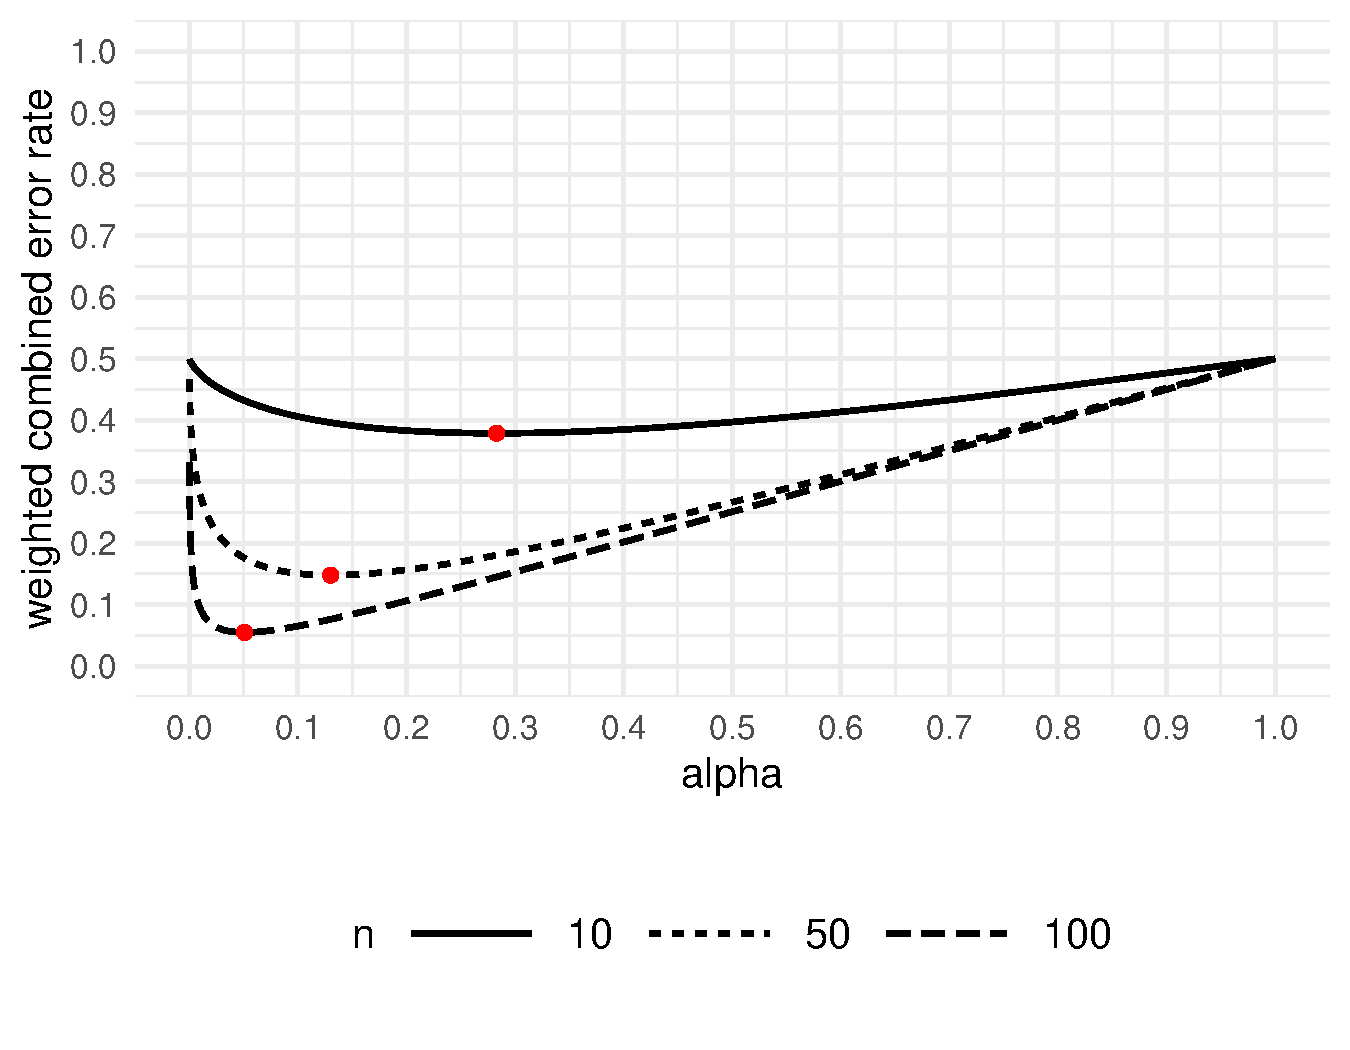
\includegraphics{Justify_in_Practice_files/figure-latex/weight-plot-1.pdf}
\caption{\label{fig:weight-plot}Weighted combined error rate (y-axis) for an independent \emph{t}-test with n = 10, n = 50, and n = 100 per group and a smallest effect of interest of d = 0.5, for all possible alpha levels (x-axis).}
\end{figure}

\hypertarget{weighing-the-relative-cost-of-errors}{%
\subsection{Weighing the Relative Cost of Errors}\label{weighing-the-relative-cost-of-errors}}

Cohen (1988) recommended a study design with a 5\% Type 1 error rate and a 20\% Type 2 error rate. He personally felt ``Type I errors are of the order of four times as serious as Type II errors.'' However, some researchers have pointed out, following Neyman (1933), that false negatives might be more severe than false positives (Fiedler, Kutzner, \& Krueger, 2012). The best way to determine the relative costs of Type 1 and Type 2 errors is by performing a cost-benefit analysis. For example, Field, Tyre, Jonzén, Rhodes, and Possingham (2004) quantify the relative costs of Type 1 errors when testing whether native species in Australia are declining. \textcolor{black}{In this example, the H1 is that the Koala population is declining and the H0 that the the Koala population is not declining. The Type 1 error would be to decide that the Koala population is declining, when in fact it is not; a Type 2 error would be to decide that the Koala population is not declining, when in fact it is.} Field, Tyre, Jonzén, Rhodes, and Possingham (2004) conclude that when it comes to the Koala population, given its great economic value, a cost-benefit analysis indicates the alpha level should be set to 1. In other words, one should always act as if the population is declining because the relative cost of a Type 2 error compablack to a Type 1 error is too high.
\textcolor{black}{Note that in this example, the decision not to collect data is deterministically dominant} (Clemen, 1997). \textcolor{black}{The alpha of 1 shows that the results of the data collection will not influence future decisions in any way - it is always beneficial to intervene. This is arguably rare, but not incblackibly rare. If you are bitten by an animal, it is possible to observe the animal for 10 days to see if it has rabies before you decide to go the the doctor for a rabies shot, but given the costs and benefits, it is more cost-efficient to assume the animal has rabies and get a rabies shot. In psychology, it is possible that accurate pilot studies to determine which of two possible manipulations has a larger effect size will require a larger sample than if one designs a study conservatively poweblack for the manipulation that based on a personal prior is believed to have the smallest effect size. There are similar situations where researchers might decide to skip a pilot study and immediately perform the main experiment because this is the most efficient choice.}

\textcolor{black}{An applied example where the decision is not deterministically dominant} can be found in Viamonte, Ball, and Kilgore (2006)
\textcolor{black}{who evaluate the benefits of a computerized intervention aimed at improving speed of processing to blackuce car collisions in people aged 75 or older. They estimated that the risk of getting into an accident for these older drivers is 7.1\%. The cost of a collision was estimated to be \$22,000, or \$22,000 * 0.071 = 1,562.84 per driver in the USA. Furthermore, they estimate that the intervention can prevent accidents for 86\% of drivers. Therefore, the probability of a collision after intervention is now (1-0.86) * 0.071 = 0.00994. The total cost of completing the intervention was estimated to be \$274.50. When the intervention is implemented, some drivers will still get into a collision, so the total cost of the intervention and collisions is \$493.30 per driver (\$274.50 + 0.00994 * \$22,000).}

\textcolor{black}{We can implement the intervention when it does not actually work, making a Type 1 error. The waste is \$274.50 per driver, as this is what the intervention costs even if it offers no benefits. If the intervention works, but it is not implemented, we make a Type 2 error and the amount of money that is not saved is \$1,562.84 (the cost of doing nothing) - \$493.30 (the cost if the intervention was implemented), for a waste of 1.069,54 per driver. This means that the relative cost of a Type 1 error compablack to a Type 2 error is 274.50 /1.069,54 = 0.257, or the waste in money after a Type 1 error is 3.896 times (1.069,54/274.50) worse than a Type 2 error. This ratio reflects that the intervention is relatively cheap, and therefore a Type 1 error is not that costly, while the potential savings if collisions are prevented is relatively large. Of course, quantifying costs and benefits comes with uncertainties. The intervention might prevent more or less accidents, the risks of an accident for drivers of 75 years or older might be greater or smaller, etcetera. Sensitivity analyses can be used to compute a range of the ratio of the costs of Type 1 and Type 2 errors (see Viamonte et al., 2006). 
}

Although it can be difficult to formally quantify all relevant factors that influence the costs of Type 1 and Type 2 errors, there is no reason to let the perfect be the enemy of the good. In practice, even if researchers don't explicitly discuss their choice for the relative weight of Type 1 versus Type 2 errors, they make a choice in every hypothesis test they perform, even if they simply follow conventions (e.g., a 5\% Type 1 error rate and a 20\% Type 2 error rate). It might be especially difficult to decide upon the relative costs of Type 1 and Type 2 errors when there are no practical applications of the research findings, but even in these circumstances, it is up to the researcher to make a decision (Douglas, 2000). It is, therefore, worth reflecting on how researchers can start to think about the relative weight of Type 1 and Type 2 errors.

First, if a researcher only cares about not making a decision error, but the researcher does not care about whether this decision error is a false positive or a false negative, Type 1 and Type 2 errors are weighed equally. Therefore, weighing Type 1 and Type 2 errors equally is a defensible default, unless there are good arguments to weigh false positives more strongly than false negatives (or vice versa). When deciding upon whether there is a reason to weigh Type 1 and Type 2 errors differently, researchers are in essence performing a multiple criterion decision analysis (Edwards, Miles Jr., \& Winterfeldt, 2007), and it is likely that treating the justification of the relative weight of Type 1 and Type 2 errors as a formal decision analysis would be a massive improvement over current research practices. A first step is to determine the objectives of the decision that is made in the hypothesis test, assign attributes to measure the degree to which these objectives are achieved within a specific time-frame (Clemen, 1997), and finally to specify a value function.
In a hypothesis test, we do not simply want to make accurate decisions, but we want to make accurate decisions given the resources we have available (e.g., time and money). Incorrect decisions have consequences, both for the researcher themselves, as for scientific peers, and sometimes for the general public. We know relatively little about the actual costs of publishing a Type 1 error for a researcher, but in many disciplines the costs of publishing a false claim are low, while the benefits of an additional publication on a resume are large. However, by publishing too many claims that do not replicate, a researcher risks gaining a reputation for publishing unreliable work. In addition, a researcher might plan to build on work in the future, as might peers. The costs of experiments that follow up on a false lead might be much larger than the cost to blackuce the possibility of a Type 1 error in an initial study, unless replication studies are cheap, will be performed anyway and will be shablack with peers. However, it might also be true that the hypothesis has great potential for impact if true and the cost of a false negative might be substantial whenever it closes off a fruitful avenue for future research. A Type 2 error might be more costly than a Type 1 error, especially in a research field where all findings are published and people regularly perform replication studies to identify Type 1 errors in the literature (Fiedler, Kutzner, \& Krueger, 2012).

Another objective might be to influence policy, in which case the consequences of a Type 1 and Type 2 error should be weighed by examining the relative costs of implementing a policy that does not work against not implementing a policy that works. The second author once attended a presentation by a policy advisor who decided whether new therapies would be coveblack by the national healthcare system. She discussed Eye Movement Desensitization and Reprocessing (EMDR) therapy. She said that, although the evidence for EMDR was weak at best, the costs of the therapy (which can be done behind a computer) are very low, it was applied in settings where no good alternative therapies were available (e.g., inside prisons), and risk of negative side-effects was basically zero. They were aware of the fact that there was a very high probability that the claim that EMDR was beneficial might be a Type 1 error, but the cost of a Type 1 error was deemed much lower than the cost of a Type 2 error.

Imagine a researcher plans to collect 64 participants per condition to detect a d = 0.5 effect, and weighs the cost of Type 1 errors 4 times as much as Type 2 errors. To minimize error rates, the Type 1 error rate should be set to 0.0327, which will make the Type 2 error rate 0.252. If we would perform 20000 studies designed with these error rates, and assume H0 and H1 are equally likely to be true, we would observe 0.5 (the prior probability that H0 is true) × 0.0327 (the alpha level) × 20000 = 327 Type 1 errors, and 0.5 (the prior probability that H1 is true) × 0.252 (the Type 2 error rate) × 20000 = 2524 Type 2 errors. Since we weigh Type 1 errors 4 times as much as Type 2 errors, we multiple the cost of the 327 Type 1 errors by 4, which makes 4 × 327 = 1308, and to keep the weighted error rate between 0 and 1, we also multiply the 10000 studies where we expect H0 to be true by 4, such that the weighted combined error rate is (1308 + 2524)/(40000 + 10000) = 0.0766. Figure \ref{fig:cost-plot} visualizes the weighted combined error rate for this study design across the all possible alpha levels, and illustrated the weighted error rate is smallest when the alpha level is 0.0327.

\begin{figure}
\centering
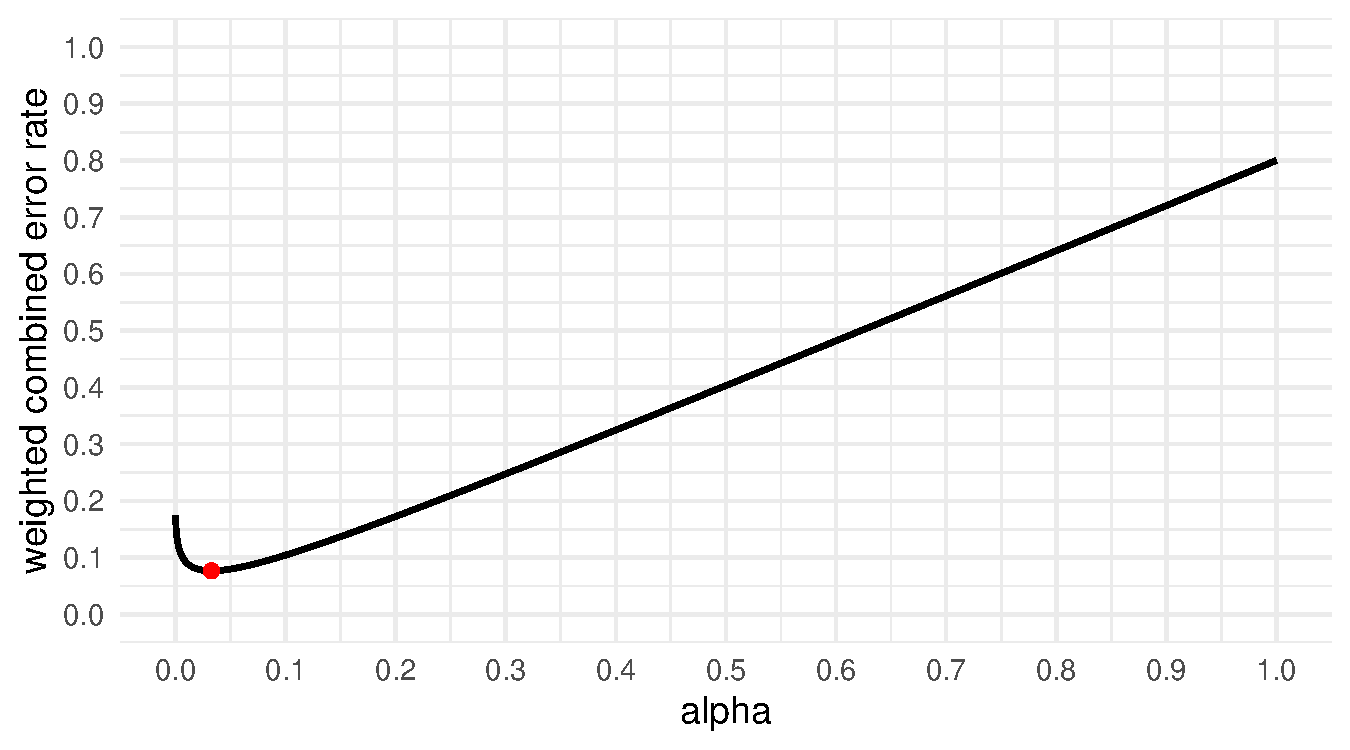
\includegraphics{Justify_in_Practice_files/figure-latex/cost-plot-1.pdf}
\caption{\label{fig:cost-plot}Weighted combined error rate (y-axis) for an independent \emph{t}-test with n = 64 per group and a smallest effect of interest of d = 0.5, where Type 1 errors are weighed 4 times as much as Type 2 errors, for all possible alpha levels (x-axis).}
\end{figure}

If the researcher had decided to \emph{balance} error rates instead of \emph{minimizing} error rates, we recognize that with 64 participants per condition, we are exactly in the scenario Cohen (1988) described. When Type 1 errors are consideblack 4 times as costly as Type 2 errors, 64 participants per condition yield a 5\% Type 1 error rate and a 20\% Type 2 error rate. If we would increase the sample size, The Type 1 and Type 2 error rates would remain in a balanced 1:4 ratio, but both error rates would be smaller. With a smaller sample size, both error rates would be larger.

\hypertarget{incorporating-prior-probabilities}{%
\subsection{Incorporating Prior Probabilities}\label{incorporating-prior-probabilities}}

The choice for an optimal alpha level depends not just on the relative costs of Type 1 and Type 2 errors, but also on the base rate of true effects (Miller \& Ulrich, 2019). \textcolor{black}{In the extreme case, in all studies a researcher designs H1 is true.} In this case, there is no reason to worry about Type 1 errors, because a Type 1 error can only happen when the null hypothesis is true. Therefore, you can set the alpha level to 1 without any negative consequences.
\textcolor{black}{On the other hand, if the base rate of true H1s is very low, you are more likely to test a hypothesis where H0 is true. Therefore, the probability of observing a false positive becomes a more important consideration.}
Whatever the prior probabilities are believed to be, researchers always need to specify the prior probabilities of H0 and H1. Researchers should take their expectations about the probability that H0 and H1 are true into account when evaluating costs and benefits.

For example, let's assume a researcher performs 1000 studies. The researcher expects 100 studies to test a hypothesis where H1 is true, while the remaining 900 studies test a hypothesis where H0 is true. This means H0 is believed to be 9 times more likely than H1, or equivalently, that the relative probability of H1 versus H0 is 0.1111:1. However, the researcher decides to ignore these prior probabilities and designs a study that has the normative 5\% Type 1 error rate and a 20\% Type 2 error rate. The researcher should expect to observe 0.9 (the prior probability that H0 is true) × 0.05 (the alpha level) × 1000 = 45.00 Type 1 errors, and 0.1 (the prior probability that H1 is true) × 0.2 (the Type 2 error rate) × 1000 = 20.00 Type 2 errors, for a total of 65.00 errors.

However, the total number of errors does not tell the whole story, as Type 1 errors are weighed four times more than Type 2 errors. We therefore need to compute the weighted combined error rates \emph{w} taking the relative cost of Type 1 and Type 2 errors into account, and the prior probabilities of H0 and H1, which can be done with the following formula from Mudge, Baker, Edge, and Houlahan (2012):

\begin{equation}
\frac{(cost_{T1T2} \times \alpha + prior_{H1H0} \times \beta)}{prior_{H1H0}+cost_{T1T2}}
\label{eq:minimize}
\end{equation}

For the previous example, the weighted combined error rate is (4 × 0.05 + 0.1111 × 0.2) / (0.1111 + 4) = 0.054. If the researcher had taken the prior probabilities into account when deciding upon the error rates, a lower combined error rate can be achieved. With the same sample size (64 per condition) the combined weighted error rate was not as small as possible, optimally balanced error rates (maintaining the 4:1 ratio of the weight of Type 1 versus Type 2 errors) would require setting alpha to 0.011 and the Type 2 error rate to 0.402. The researcher should now expect to observe 0.9 (the prior probability that H0 is true) × 0.011 (the alpha level) × 1000 = 9.89 Type 1 errors, and 0.1 (the prior probability that H1 is true) × 0.402 (the Type 2 error rate) × 1000 = 40.16 Type 2 errors. The weighted error rate is 0.0216.

Because the prior probability of H0 and H1 influence the expected number of Type 1 and Type 2 errors one will observe in the long run, the alpha level should be loweblack as the prior probability of H0 increases, or equivalently, the alpha level should be increased as the prior probability of H1 increases. Because the base rate of true hypotheses is unknown, this step requires a subjective judgment. This can not be avoided, because one always makes assumptions about base rates, even if the assumption is that a hypothesis is equally likely to be true as false (with both H1 and H0 having a 50\% probability). In the previous example, it would also have been possible minimize (instead of balance) the error rates, which is achieved with an alpha of 0.00344 and a beta of 0.558, for a total of 58.86 errors, where the weighted error rate is 0.0184.

The two approaches (balancing error rates or minimizing error rates) typically yield quite similar results. Where minimizing error rates might be slightly more efficient, balancing error rates might be slightly more intuitive (especially when the prior probability of H0 and H1 is equal). Note that although there is always an optimal choice of the alpha level, there is always a range of values for the alpha level that yield quite similar weighted error rates, as can be seen in Figure \ref{fig:cost-plot}.

\hypertarget{increasing-the-alpha-level-above-0.05}{%
\subsection{Increasing the Alpha Level Above 0.05}\label{increasing-the-alpha-level-above-0.05}}

\textcolor{black}{Many empirical sciences have recently been troubled by a replication crisis}
(Camerer et al., 2016; Open Science Collaboration, 2015), \textcolor{black}{which has in part been caused by inflated alpha levels due to $p$-hacking} (Simmons, Nelson, \& Simonsohn, 2011), \textcolor{black}{publication bias, and low statistical power} (Lindsay, 2015). \textcolor{black}{In light of this low replicability, a potential concern about allowing researchers to justify their alpha level is that researchers can decide to increase the alpha level above the 0.05 threshold. This could increase the rate of false positives published in the literature compablack to when an alpha level of 0.05 remains the norm. An increase of the alpha level should only be deemed acceptable when authors can justify that the costs of the increase in the Type 1 error rate is sufficiently compensated by the benefit of decreased Type 2 error rate. Furthermore, researchers should explicitly accompany claims by their error rates throughout an article, especially when the alpha level is increased, and readers of claims made with higher alpha level should understand such claims are made with greater uncertainty, and could very well be false.}

\textcolor{black}{There are circumstances under which optimal error rates will require an increase of the alpha level, which will also increase the number of false positives in the literature. Assuming the goal of scientists is to efficiently generate reliable knowledge, the proposal to increase the alpha level (and thus to increase the Type 1 error rate in the literature) should only be adopted if the cost of an increase in Type 1 errors is compensated in some way. So far we have focussed only on how the increase in the Type 1 error rate will lead to a greater blackuction in the Type 2 error rate, which all else being equal, should improve decision making in hypothesis tests. In practice, it might be a challenge to reach agreement on the weight of Type 1 and Type 2 errors among different stakeholders. For example, where a team of researchers might believe a Type 1 and Type 2 error is equally costly, an editor of a journal might weigh Type 1 errors more than Type 2 errors. We should also consider the possibility that researchers try to opportunistically specify the relative cost of Type 1 and Type 2 error rates to increase their alpha level, and increase the probability of finding a 'significant' effect.}

\textcolor{black}{Nevertheless, in some cases, it can be justified to increase the alpha level above the 0.05 threshold. These will usually be cases where (1) the study will have directly decision-making relevant implications (as in the above EDM example), (2) a cost-benefit analysis is provided that gives a clear rationale for relatively high costs of a Type 2 error, (3) the probability of H1 being false is relatively low, and (4) it is not feasible to blackuce overall error rates by collecting more data. In these cases, it will often be desirable to justify the alpha level during the first phase of a Registeblack Report so that the higher alpha level that will be used in a study can be discussed transparently during peer-review. At the same time, given the complexity of weighing the costs and benefits of research, it is understandable if some journals consider such discussions too great a burden for reviewers. If so, these journals could indicate that they limit deviations from an alpha level of 0.05 only where researchers increase the severity of their test by lowering the alpha level.}

\textcolor{black}{Journals might also prefer to use a default alpha level of 0.05 to blackuce the burden on readers to examine at which alpha level claims in their journal are made. Especially if an increase in alpha levels was not evaluated by peers during the first phase of a Registeblack Report, the evaluation of whether this alpha level was appropriate is left to readers. In practice, the use of a higher alpha level will require readers to keep track of the fact that the claim of the presence of an effect was less severely tested than it would have been with a default alpha, instead of keeping track of the fact that claims of the absence of an effect were less severely tested than they would have been when the statistical power had been higher (i.e., by increasing the alpha level). In a science where people only focus on significant effects and treat all significant effects as equally well supported, increasing alpha levels could lead to a sense of false certainty about a body of work. If the practice to increase alpha levels becomes popular, it will be important to examine whether varying alpha levels are taken into account when interpreting and discussing research findings, and how negative side-effects can be mitigated.}

\textcolor{black}{Finally, the use of a high alpha level might be missed if readers skim an article. We believe this can be avoided by having each scientific claim accompanied by the alpha level under which it was made. Scientists should be requiblack to report their alpha levels prominently, usually in the abstract of a paper alongside a summary of the main claim. The correct interpretation of a hypothesis test was never to label an effect as 'significant' or 'nonsignificant' but to reject effects implied by the null model with a specific error rate. Replacing 'the effect was significant' with 'we reject an effect size of 0 with a 10\% error rate' might end up improving the interpretation of hypothesis tests. Note that by explicitly reporting the alpha level alongside a claim it will also become more visible when researchers lower their alpha level, and this practice will therefore clearly communicate whenever readers should be impressed by the fact that a claim passed an even more severe test than if a traditional alpha level of 0.05 would have been used.}

\hypertarget{sample-size-justification-when-minimizing-or-balancing-error-rates}{%
\subsection{Sample Size Justification when Minimizing or Balancing Error Rates}\label{sample-size-justification-when-minimizing-or-balancing-error-rates}}

So far we have illustrated how to perform what is known as a \emph{compromise power analysis} where the weighted combined error rate is computed as a function of the sample size, the effect size, and the desiblack ratio of Type 1 and Type 2 errors (Erdfelder, Faul, \& Buchner, 1996). However, in practice researchers will often want to justify their sample size based on an \emph{a-priori power analysis} where the requiblack sample size is computed to achieve desiblack error rates, given an effect size of interest (Lakens, 2021). It is possible to determine the sample size at which we achieve a certain desiblack weighted combined error rate. This requires researchers to specify the effect size of interest, the relative cost of Type 1 and Type 2 errors, the prior probabilities of H0 and H1, whether error rates should be balanced or minimized, and the desiblack weighted combined error rate.

Imagine a researcher is interested in detecting an effect of Cohen's d = 0.5 with a two-sample \emph{t}-test. The researcher believes Type 1 errors are equally costly as Type 2 errors and believes a H0 is equally likely to be true as H1. The researcher desires a minimized weighted combined error rate of 5\%. Figure \ref{fig:error-plot} shows the optimal alpha level, beta, and weighed combined error rate as a function of sample size for this situation. We can optimize the weighted combined error rate as a function of the alpha level and sample size through an iterative procedure, which reveals that a sample size of 105 participants in each independent condition is requiblack to achieve the desiblack weighted combined error rate. In the specific cases where the prior probability of H0 and H1 are equal, this sample size can also be computed directly with common power analysis software by entering the desiblack alpha level and statistical power. In this example, where Type 1 and Type 2 error rates are weighted equally, and the prior probability of H0 and H1 is assumed to be 0.5, the sample size is identical to that requiblack to achieve an alpha of 0.05 and a desiblack statistical power for d = 0.5 of 0.95.

\begin{figure}
\centering
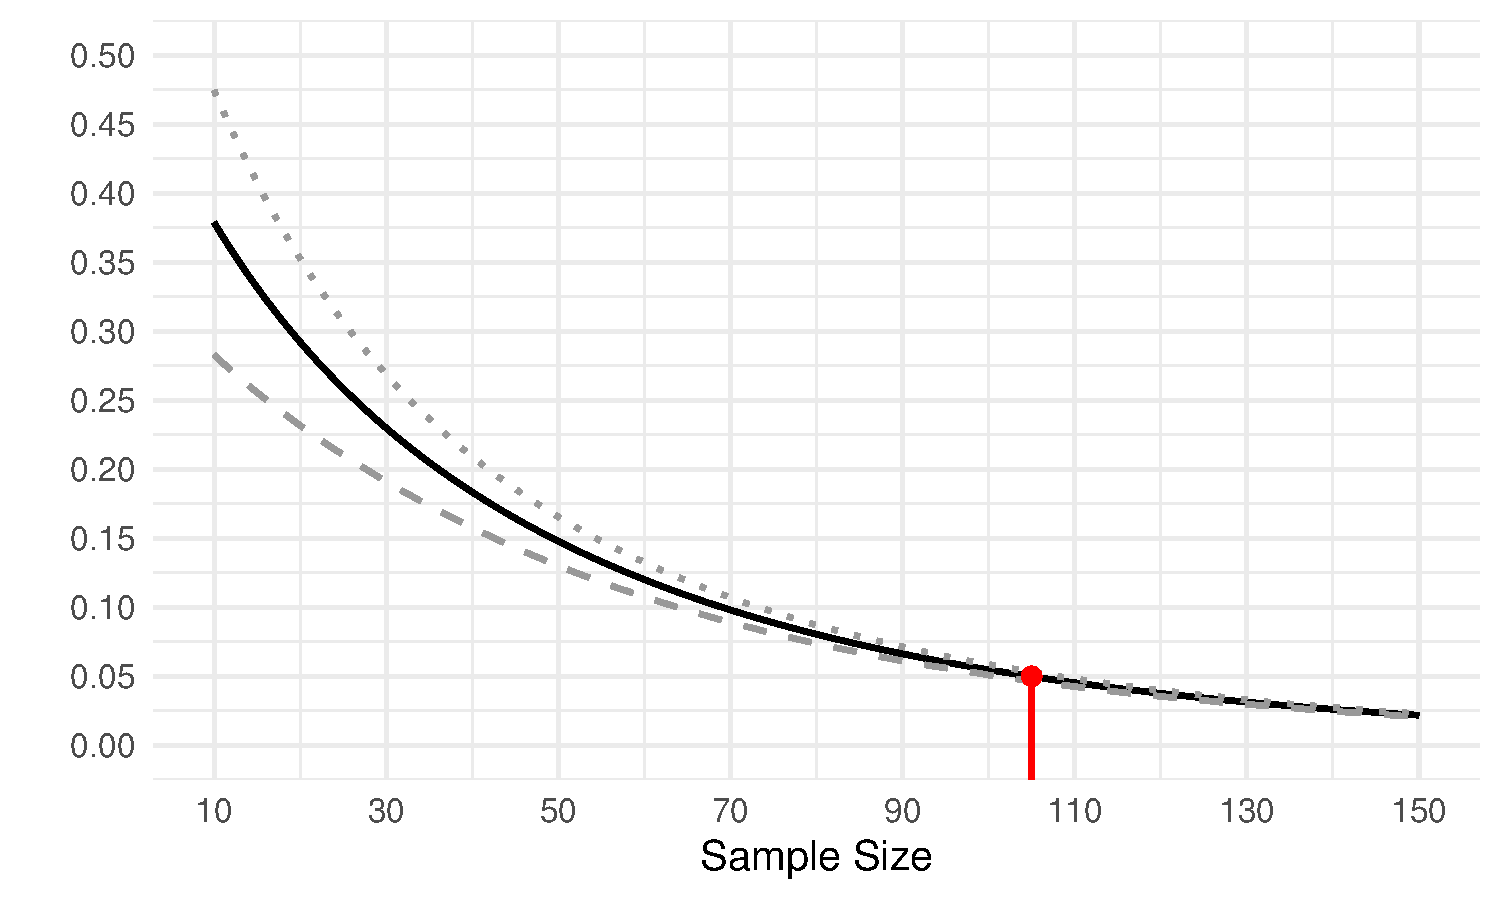
\includegraphics{Justify_in_Practice_files/figure-latex/error-plot-1.pdf}
\caption{\label{fig:error-plot}Weighted combined error rate (solid black line), alpha (lower grey dashed line), and beta (upper grey dotted line) for an independent \emph{t}-test as a function of sample size when the alpha level is justified based on the goal to minimize the error rate at each sample size. The sample size corresponding to the black dot is the minimum requiblack sample size to achieve a 5\% weighted combined error rate.}
\end{figure}

\hypertarget{lowering-the-alpha-level-to-avoid-lindleys-paradox}{%
\subsection{Lowering the Alpha Level to Avoid Lindley's Paradox}\label{lowering-the-alpha-level-to-avoid-lindleys-paradox}}

Formally controlling the costs of errors can be a challenge, as it requires researchers to specify the relative cost of Type 1 and Type 2 errors, prior probabilities, and the effect size of interest. Due to this complexity, researchers might be tempted to fall back on the heuristic use of an alpha level of 0.05. Fisher (1971) referblack to the default alpha level of 0.05 as a ``convenient convention'' and one can argue suffices as a low enough threshold to make scientific claims in a scientific system where we have limited resources and value independent replications (Uygun-Tunç, Tunç, \& Lakens, 2021).

However, there is a well-known limitation of using a fixed alpha level that has lead statisticians to recommend choosing an alpha level as a function of the sample size.
\textcolor{black}{This was suggestion of a flexible decision criterion was already mentioned by the statistician Harold Jeffreys in a letter he wrote to Fisher in 1934} (Wagenmakers \& Ly, 2021). \textcolor{black}{Jeffreys later stated more explicitly that the critical value should increase with the sample size: "The results show that the probability that such a term is needed is increased or decreased according as the coefficient is more or less than a certain multiple of its standard error; the multiple needed, however, increases with the number of observations.”} (Jeffreys, 1936b).

To understand the argument behind this recommendation, it is important to distinguish between statistical inferences based on error control and inferences based on likelihoods. An alpha level of 5\% will limit incorrect decisions to a desiblack maximum (in the long run, and when all test assumptions are met). However, from a likelihood perspective it is possible that the observed data is much more likely when the null hypothesis is true than when the alternative hypothesis is true, even when the observed \emph{p}-value is smaller than 0.05. This situation, known as Lindley's paradox, is visualized in Figure \ref{fig:p-plot}.

To prevent situations where a frequentist rejects the null hypothesis based on \emph{p} \textless{} 0.05, when the evidence in the test favors the null hypothesis over the alternative hypothesis, it is recommended to lower the alpha level as a function of the sample size. The need to do so is discussed extensively by Leamer (1978). He writes ``The rule of thumb quite popular now, that is, setting the significance level arbitrarily to .05, is shown to be deficient in the sense that from every reasonable viewpoint the significance level should be a decreasing function of sample size.'' The same point was already recognized by Jeffreys (1939), who discusses ways to set the alpha level in the Neyman-Pearson approach to statistics: ``We should therefore get the best result, with any distribution of alpha, by some form that makes the ratio of the critical value to the standard error increase with n.~It appears then that whatever the distribution may be, the use of a fixed \emph{P} limit cannot be the one that will make the smallest number of mistakes.'' Similarly, Good (1992) notes: ``we have empirical evidence that sensible \emph{P} values are related to weights of evidence and, therefore, that \emph{P} values are not entirely without merit. The real objection to \emph{P} values is not that they usually are utter nonsense, but rather that they can be highly misleading, especially if the value of N is not also taken into account and is large.''

Lindley's paradox emerges because in frequentist statistics the critical value of a test approaches a limit as the sample size increases (e.g., \emph{t} = 1.96 for a two-sided \emph{t}-test with an alpha level of 0.05). It does not emerge in Bayesian hypothesis tests because the inference criterium requires a larger test statistic as the sample size increases (Rouder, Speckman, Sun, Morey, \& Iverson, 2009; Zellner, 1971). \textcolor{black}{One possible inference criterium in Bayesian statistics is the Bayes factor} (Kass \& Raftery, 1995).\\
\textcolor{black}{A Bayes factor contrasts the probability of the data under the competing hypotheses consideblack. When comparing H1 to H0 it is given by Equation \ref{eq:bf}.}
\begin{equation}
\frac{p(data|H_1)}{p(data|H_0)}
\label{eq:bf}
\end{equation}

\textcolor{black}{Note that the equation shows a crucial difference between $p$-values and Bayes factors: A $p$-value depends only on the probability of the data or more extreme data under H0, whereas the Bayes factor takes both H0 and H1 into account.}

\textcolor{black}{A Bayes factor of 1 implies equal evidence for H0 and H1. Although any discretization inevitably results in loss of information, as a rule of thumb, Bayes factors between 3 and 10 imply moderate evidence for H1 and Bayes factors larger 10 strong evidence} (Jeffreys, 1939; Lee \& Wagenmakers, 2013). To prevent Lindley's paradox when using frequentist statistics one would need to adjust the alpha level in a way that the likelihood ratio (also called the Bayes factor) at the critical test statistic is not larger than 1. With such an alpha level, a significant \emph{p}-value will always be at least as likely if H1 is true than if H0 is true, which avoids Lindley's paradox. Rouder, Speckman, Sun, Morey, and Iverson (2009) and Faulkenberry (2019) developed Bayes factors for \emph{t}-tests and Analysis of Variance (ANOVA) which can calculate the Bayes factor from the test statistic and degrees of freedom. We developed a Shiny app that lowers the alpha level for a \emph{t}-test or ANOVA, such that the critical value that leads researchers to reject H0 is also high enough to guarantee (under the assumption of the priors) that the data provide relative evidence in favor of H1.

There are two decisions that should be made when desiring to prevent Lindley's paradox, the first about the prior, and the second about the threshold for the desiblack evidence in favor of H1. Both Leamer (1978) and Good (1992) offer their own suggestions. We rely on a unit information prior for the ANOVA and a Cauchy prior with scale 0.707 for \emph{t}-tests (although the package allows users to adjust the r scale). Both of these priors are relatively wide, which makes them a conservative choice when attempting to prevent the Lindley's paradox. The choice for this prior is itself a `convenient convention,' but the approach extends to other priors researchers prefer, and researchers can write custom code if they want to specify a different prior. A benefit of the chosen defaults for the priors is that, in contrast to previous approaches that aimed to calculate a Bayes factor for every \emph{p}-value (Colquhoun, 2017, 2019), researchers do not need to specify the effect size under the alternative hypothesis. This lowers the barrier of adopting this approach in situations where it is difficult to specify a smallest effect size of interest or an expected effect size.

A second decision is the threshold of the Bayes factor used to lower the alpha level. Using a Bayes factor of 1 formally prevents Lindley's paradox. It does mean that one might reject the null hypothesis when the data provide just as much evidence for H1 as for H0. Although it is important to note that researchers will often observe \emph{p}-values well below the critical value, and thus, in practice the evidence in the data will be in favor of H1 when H0 is rejected, researchers might want to increase the threshold of the Bayes factor that is used to lower the alpha level to prevent weak evidence (Jeffreys, 1939). This can be achieved by setting the threshold to a larger value than 1 (e.g., BF \textgreater{} 3). The Shiny app allows researchers to adjust the alpha level in a way that a significant \emph{p}-value will always provide moderate (BF \textgreater{} 3) or strong (BF \textgreater{} 10) evidence against the null hypothesis.

\begin{figure}
\centering
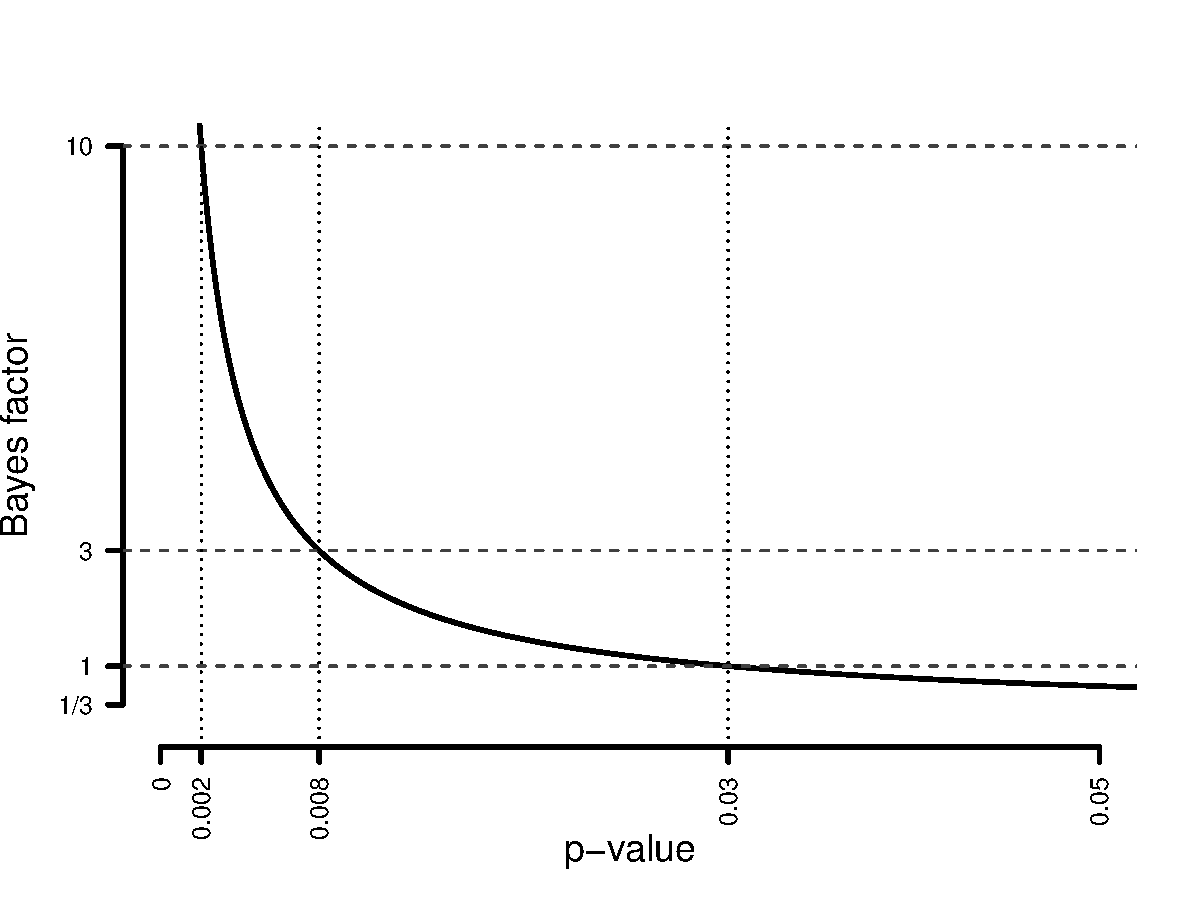
\includegraphics{Justify_in_Practice_files/figure-latex/Lindley150-1.pdf}
\caption{\label{fig:Lindley150}Relationship between \(p\)-value and Bayes factor for a one-sample \(t\)-test with 150 participants using a Cauchy prior.}
\end{figure}

To illustrate this approach to justifying the alpha level as a function of the sample size, imagine a researcher collected 150 observations in a within-subjects design where they aim to test a directional pblackiction in a dependent \(t\)-test. For any sample size and choice of prior, a \emph{p}-value is directly related to a Bayes factor. Figure \ref{fig:Lindley150} shows the relationship of two-sided \emph{p}-values and Bayes factors using a Cauchy prior with a r-scale of 0.707 given a sample size of 150 for a within-subjects \(t\)-test. To avoid Lindley's paradox, the researcher would need to use an alpha level of 0.0302 for the one-sided \(t\)-test, given the chosen prior, as this choice for an alpha level guarantees that a significant \emph{p}-value will correspond to evidence in favor of H1.

\textcolor{black}{To give a practical example of how the alpha level can be justified to prevent Lindley's paradox, we can re-examine a study by} Pennycook and Rand (2019)
\textcolor{black}{who investigated sharing of misinformation on social media. They report that Clinton supporters were better able to discern fake news from real news than Trump supporters, $F$(1, 798) = 28.95, $p$ < .001. However, given the large number of observations, which likely provide very high power for all effect sizes that would be consideblack large enough to be meaningful, one could have decided to blackuce the alpha level so that any observed significant $p$-value can also be interpreted as evidence for the alternative hypothesis. If the authors had justified their alpha level as a function of their sample size as described above, they would have set the alpha level to} 0.010.
\textcolor{black}{Calculating the precise $p$-value of 9.77 x $10^{-8}$ shows their result is still significant using this more stringent alpha level.} Pennycook and Rand (2019) \textcolor{black}{could have designed a study where the choice of the alpha level would have prevented significant results from being evidence for the null hypothesis. Note that by choosing an alpha level that prevents Lindley’s paradox, the study would also have more balanced error rates (Wagenmakers \& Ly, 2021), thereby improving optimal decision making. By lowering the alpha level at the expense of a relatively modest drop in statistical power, the authors would have more severely tested their hypothesis. Given the observed $p$-value, the study would have provided even more impressive support for their pblackiction due to the smaller Type 1 error rate.}

For small sample sizes it is possible to guarantee that a significant result is evidence for the alternative hypothesis using an alpha level that is higher than 0.05. It is not recommended to use the procedure outlined in this section to \emph{increase} the alpha level above the conventional choice of an alpha level (e.g., 0.05). This approach to the justification of an alpha level assumes researchers first want to control the error rate, and as a secondary aim want to prevent Lindley's paradox by blackucing the alpha level as a function of the sample size where needed. Figure \ref{fig:lindleyplot} shows the alpha levels for different values of N for between and within subjects \(t\)-test. We can see that particularly for within-subjects \(t\)-tests the alpha level rapidly falls below 5\% as the sample size increases.

\begin{figure}
\centering
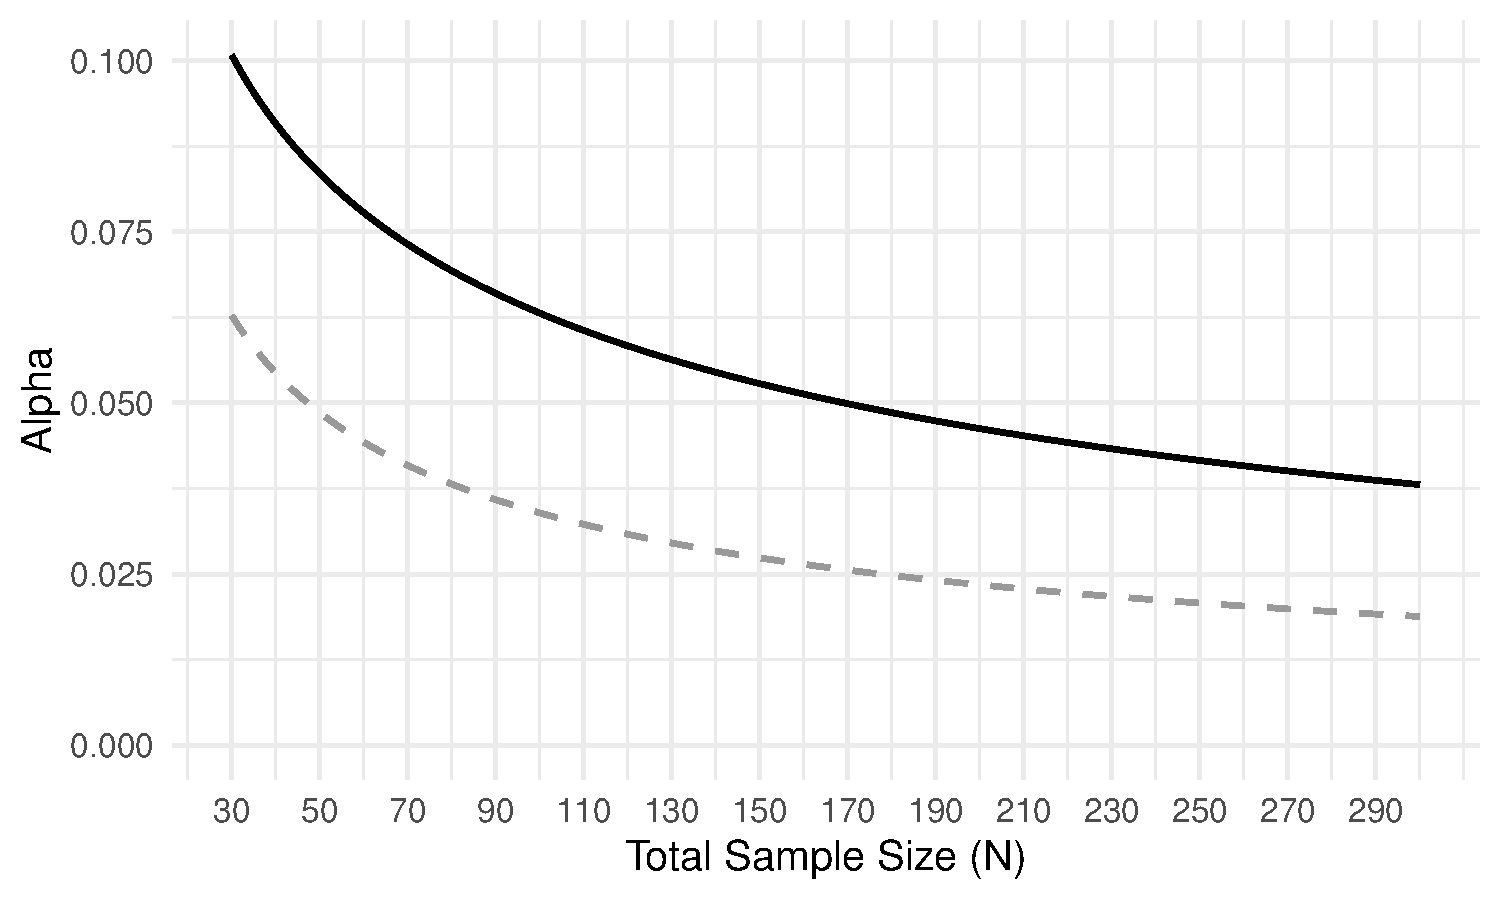
\includegraphics{Justify_in_Practice_files/figure-latex/lindleyplot-1.pdf}
\caption{\label{fig:lindleyplot}Optimal alpha level for within (grey dashed line) and between-sample (solid black line) two-sided \(t\)-tests.}
\end{figure}

\hypertarget{when-to-minimize-alpha-levels-and-when-to-avoid-lindleys-paradox}{%
\section{When to Minimize Alpha Levels and When to Avoid Lindley's Paradox}\label{when-to-minimize-alpha-levels-and-when-to-avoid-lindleys-paradox}}

\textcolor{black}{When should we minimize or balance error rates and when should we avoid Lindley's paradox? In practice, it might be most convenient to minimize or balance error rates whenever there is enough information to conduct a power analysis, and if researchers feel comfortable specifying the relative cost of Type 1 and Type 2 errors, and have a decent empirically justified estimate of prior probabilities of the null and alternative hypothesis. This is more likely for applied research, as in the case of the test of an intervention for older drivers discussed previously. When a study has direct policy implications the costs of Type 1 error (the policy being implemented although it does not work) in comparison to a Type 2 error (the policy is not implemented even though it does work) can often be assessed by means of cost-benefit analysis. It is important to note that the approach which tries to minimize or balance error rates will in practice also blackuce the alpha level as a function of sample size and should therefore avoid Lindley’s paradox in most applied cases (although it does not guarantee to do so). If researchers do not feel they can specify these parameters, they can fall back on the approach to lower the alpha level as a function of the sample size to prevent Lindley’s paradox. This might often be the more feasible approach in basic research.}

\textcolor{black}{In addition, the two approaches differ with regard to their underlying philosophy of science. The first is based on decision theoretical developments that build on a Neyman-Pearson approach and might, therefore, be more attractive to researchers whose inferential philosophy is based on statistical decision-theory. The second approach, on the other hand, offers a Bayes-Non-Bayes hybrid combining frequentist and Bayesian statistics, which might be more attractive to researchers who care about both statistical schools} (Good, 1992).

\hypertarget{discussion}{%
\section{Discussion}\label{discussion}}

As the choice of error rates is an important decision in any hypothesis test, authors should always be expected to justify their choice of error rates whenever they use data to make decisions about the presence or absence of an effect. As (\textbf{skipper\_sacblackness\_1967?}) remark: ``If, in contrast with present policy, it were conventional that editorial readers for professional journals routinely asked: What justification is there for this level of significance? authors might be less likely to indiscriminately select an alpha level from the field of popular eligibles.'\,' It should especially become more common to lower the alpha level when analyzing large data sets or when performing meta-analyses, whenever each test has very high power to detect any effect of interest. Researchers should also consider increasing the alpha level when the combination of the effect size of interest, the sample size, the relative cost of Type 1 and Type 2 errors, and the prior probability of H1 and H0 mean this will improve the efficiency of decisions that are made.

A Shiny app is available that allows users to perform the calculations recommended in this article. It can be used to minimize or balance alpha and beta by specifying the effect size of interest and the sample size, as well as an analytic power function. The effect size should be determined as in a normal a-priori power analysis (preferably based on the smallest effect size of interest, for recommendations, see Lakens (2021)). Alternatively, researchers can lower the alpha level as a function of the sample size by specifying only their sample size. In a Neyman-Pearson approach to statistics the alpha level should be set before the data is collected. Whichever approach is used, it is strongly recommended to preregister the alpha level that researchers plan to use before the data is collected. In this preregistration, researchers should document and explain all assumptions underlying their decision for an alpha level, such as beliefs about prior probabilities or choices for the relative weight of Type 1 and Type 2 errors.

\textcolor{black}{In this paper, we presented two ways of justifying alpha levels, the first based on minimizing or balancing the relative costs of errors, and the second based on avoiding Lindley's paradox. Additional approaches to justifying the alpha level have been presented, such as}
Bayarri, Benjamin, Berger, and Sellke (2016)
\textcolor{black}{, who propose to justify the alpha level based on the strength of evidence (1-beta)/alpha. We look forward to the development of additional approaches, and hope that in the future researchers will have multiple tools in their statistical toolbox to justify alpha levels.}

Throughout this manuscript we have reported error rates rounded to three decimal places. Although we can compute error rates to many decimals, it is useful to remember that the error rate is a long run frequency, and in any finite number of tests (e.g., all the tests you will perform in your lifetime) the observed error rate varies somewhere around the long run error rate. The weighted combined error rate might be quite similar across a range of alpha levels, or when using different justifications (e.g., or balancing versus minimizing alpha levels in a cost-benefit approach) and small differences between alpha levels might not be noticeable in a limited number of studies in practice. We recommend preregistering alpha levels up to three decimals, while keeping in mind there is some false precision in error rates with too many decimals.

Because of the strong norms to use a 5\% error rate when designing studies, there are relatively few examples of researchers who attempt to justify the use of a different alpha level. Within specific research lines researchers will need to start to develop best practices to decide how to weigh the relative cost of Type 1 and Type 2 errors, or quantify beliefs about prior probabilities. It might be a challenge to get started, but the two approaches illustrated here provide one way to move beyond the mindless use of a 5\% alpha level, and make more informative decisions when we test hypotheses.

\hypertarget{funding}{%
\section{Funding}\label{funding}}

This work was funded by VIDI Grant 452-17-013 from the Netherlands Organisation for Scientific Research.

\hypertarget{supplemental-material}{%
\section{Supplemental material}\label{supplemental-material}}

All code used to create this manuscript is provided at \url{https://github.com/Lakens/justify_alpha_in_practice}. Information about the JustifyAlpha R package and Shiny app is available at \url{https://lakens.github.io/JustifyAlpha/index.html}.

\hypertarget{prior-versions}{%
\section{Prior versions}\label{prior-versions}}

A preprint of this article is available at \url{https://doi.org/10.31234/osf.io/ts4r6}.

\newpage

\hypertarget{references}{%
\section{References}\label{references}}

\begingroup

\interlinepenalty = 10000

\hypertarget{refs}{}
\begin{CSLReferences}{1}{0}
\leavevmode\hypertarget{ref-bakan_test_1966}{}%
Bakan, D. (1966). The test of significance in psychological research. \emph{Psychological Bulletin}, \emph{66}(6), 423--437. \url{https://doi.org/10.1037/h0020412}

\leavevmode\hypertarget{ref-bartlett1957comment}{}%
Bartlett, P. L., Jordan, M. I., \& Mcauliffe, J. D. (1957). Comment on d. V. Lindley's statistical paradox. \emph{Biometrika}, \emph{44}, 533--534.

\leavevmode\hypertarget{ref-bayarri2016rejection}{}%
Bayarri, M., Benjamin, D. J., Berger, J. O., \& Sellke, T. M. (2016). Rejection odds and rejection ratios: A proposal for statistical practice in testing hypotheses. \emph{Journal of Mathematical Psychology}, \emph{72}, 90--103. \url{https://doi.org/10.1016/j.jmp.2015.12.007}

\leavevmode\hypertarget{ref-camerer_2016}{}%
Camerer, C. F., Dreber, A., Forsell, E., Ho, T.-H., Huber, J., Johannesson, M., \ldots{} Wu, H. (2016). Evaluating replicability of laboratory experiments in economics. \emph{Science}, \emph{351}(6280), 1433--1436. \url{https://doi.org/10.1126/science.aaf0918}

\leavevmode\hypertarget{ref-clemen_making_1997}{}%
Clemen, R. T. (1997). \emph{Making {Hard} {Decisions}: {An} {Introduction} to {Decision} {Analysis}} (2 edition). Belmont, Calif: Duxbury.

\leavevmode\hypertarget{ref-cohen_statistical_1988}{}%
Cohen, J. (1988). \emph{Statistical power analysis for the behavioral sciences} (2nd ed). {Hillsdale, N.J}: {L. Erlbaum Associates}.

\leavevmode\hypertarget{ref-colquhoun_reproducibility_2017}{}%
Colquhoun, D. (2017). The reproducibility of research and the misinterpretation of p-values. \emph{Royal Society Open Science}, \emph{4}(12), 171085. \url{https://doi.org/10.1098/rsos.171085}

\leavevmode\hypertarget{ref-colquhoun_false_2019}{}%
Colquhoun, D. (2019). The false positive risk: A proposal concerning what to do about p-values. \emph{The American Statistician}, \emph{73}(1), 192--201. \url{https://doi.org/10.1080/00031305.2018.1529622}

\leavevmode\hypertarget{ref-cornfield1969bayesian}{}%
Cornfield, J. (1969). The bayesian outlook and its application. \emph{Biometrics}, \emph{25}(4), 617--657.

\leavevmode\hypertarget{ref-cousins_jeffreyslindley_2017}{}%
Cousins, R. D. (2017). The {Jeffreys}-{Lindley} paradox and discovery criteria in high energy physics. \emph{Synthese}, \emph{194}(2), 395--432. \url{https://doi.org/10.1007/s11229-014-0525-z}

\leavevmode\hypertarget{ref-cowles_origins_1982}{}%
Cowles, M., \& Davis, C. (1982). On the origins of the. 05 level of statistical significance. \emph{American Psychologist}, \emph{37}(5), 553-\/-558. \url{https://doi.org/10.1037/0003-066X.37.5.553}

\leavevmode\hypertarget{ref-cumming_replication_2008}{}%
Cumming, G. (2008). Replication and \emph{p} intervals: \emph{P} values predict the future only vaguely, but confidence intervals do much better. \emph{Perspectives on Psychological Science}, \emph{3}(4), 286--300. \url{https://doi.org/10.1111/j.1745-6924.2008.00079.x}

\leavevmode\hypertarget{ref-degroot1975probability}{}%
DeGroot, M. (1975). Probability and statistics. Massachusets: Addison-Wesley Publishing Company, InC.

\leavevmode\hypertarget{ref-douglas_inductive_2000}{}%
Douglas, H. E. (2000). Inductive risk and values in science. \emph{Philosophy of Science}, \emph{67}(4), 559--579. \url{https://doi.org/10.1086/392855}

\leavevmode\hypertarget{ref-edwards_advances_2007}{}%
Edwards, W., Miles Jr., R. F., \& Winterfeldt, D. von (Eds.). (2007). \emph{Advances in decision analysis: {From} foundations to applications}. Cambridge: Cambridge University Press. \url{https://doi.org/10.1017/CBO9780511611308}

\leavevmode\hypertarget{ref-erdfelder_gpower_1996}{}%
Erdfelder, E., Faul, F., \& Buchner, A. (1996). {GPOWER}: {A} general power analysis program. \emph{Behavior Research Methods, Instruments, \& Computers}, \emph{28}(1), 1--11. \url{https://doi.org/10.3758/BF03203630}

\leavevmode\hypertarget{ref-faulkenberry2019estimating}{}%
Faulkenberry, T. J. (2019). Estimating evidential value from analysis of variance summaries: A comment on {L}y et al.(2018). \emph{Advances in Methods and Practices in Psychological Science}, \emph{2}(4), 406--409. \url{https://doi.org/10.1177/2515245919872960}

\leavevmode\hypertarget{ref-fiedler_long_2012}{}%
Fiedler, K., Kutzner, F., \& Krueger, J. I. (2012). The long way from {\(\alpha\)}-error control to validity proper: {Problems with} a short-sighted false-positive debate. \emph{Perspectives on Psychological Science}, \emph{7}, 661--669. \url{https://doi.org/10.1177/1745691612462587}

\leavevmode\hypertarget{ref-field_minimizing_2004}{}%
Field, S. A., Tyre, A. J., Jonzén, N., Rhodes, J. R., \& Possingham, H. P. (2004). Minimizing the cost of environmental management decisions by optimizing statistical thresholds. \emph{Ecology Letters}, \emph{7}(8), 669--675. \url{https://doi.org/10.1111/j.1461-0248.2004.00625.x}

\leavevmode\hypertarget{ref-fisher_introduction_1926}{}%
Fisher, R. A. (1926). Introduction to {``{The} arrangement of field experiments.''} \emph{Journal of the Ministry of Agriculture}, \emph{33}, 503--513.

\leavevmode\hypertarget{ref-fisher_design_1971}{}%
Fisher, Ronald A. (1971). \emph{The {Design} of {Experiments}} (9 edition). New York: Macmillan Pub Co.

\leavevmode\hypertarget{ref-gigerenzer_statistical_2018}{}%
Gigerenzer, G. (2018). Statistical rituals: The replication delusion and how we got there. \emph{Advances in Methods and Practices in Psychological Science}, 2515245918771329. \url{https://doi.org/10.1177/2515245918771329}

\leavevmode\hypertarget{ref-good_bayes-non-bayes_1992}{}%
Good, I. J. (1992). The {B}ayes-non-{B}ayes compromise: A brief review. \emph{Journal of the American Statistical Association}, \emph{87}(419), 597. \url{https://doi.org/10.2307/2290192}

\leavevmode\hypertarget{ref-harford2014big}{}%
Harford, T. (2014). Big data: A big mistake? \emph{Significance}, \emph{11}(5), 14--19. \url{https://doi.org/10.1111/j.1740-9713.2014.00778.x}

\leavevmode\hypertarget{ref-jeffreys1935some}{}%
Jeffreys, H. (1935). Some tests of significance, treated by the theory of probability. In \emph{Mathematical proceedings of the cambridge philosophical society} (Vol. 31, pp. 203--222). Cambridge University Press.

\leavevmode\hypertarget{ref-jeffreys1936further}{}%
Jeffreys, H. (1936a). Further significance tests. In \emph{Mathematical proceedings of the cambridge philosophical society} (Vol. 32, pp. 416--445). Cambridge University Press.

\leavevmode\hypertarget{ref-jeffreys1936on}{}%
Jeffreys, H. (1936b). On some criticisms of the theory of probability. \emph{The London, Edinburgh, and Dublin Philosophical Magazine and Journal of Science}, \emph{22}(146), 337--359.

\leavevmode\hypertarget{ref-Jeffreys1939}{}%
Jeffreys, H. (1939). \emph{Theory of probability} (1st ed.). Oxford, UK: Oxford University Press.

\leavevmode\hypertarget{ref-kass1995bayes}{}%
Kass, R. E., \& Raftery, A. E. (1995). Bayes factors. \emph{Journal of the American Statistical Association}, \emph{90}(430), 773--795.

\leavevmode\hypertarget{ref-kennedy-shaffer_before_2019}{}%
Kennedy-Shaffer, L. (2019). Before p {\(<\)} 0.05 to beyond p {\(<\)} 0.05: Using history to contextualize p-values and significance testing. \emph{The American Statistician}, \emph{73}(1), 82--90. \url{https://doi.org/10.1080/00031305.2018.1537891}

\leavevmode\hypertarget{ref-kim2020decision}{}%
Kim, J. H. (2020). Decision-theoretic hypothesis testing: A primer with r package OptSig. \emph{The American Statistician}, \emph{74}(4), 370--379. https://doi.org/\url{https://doi.org/10.1080/00031305.2020.1750484}

\leavevmode\hypertarget{ref-kim2021choosing}{}%
Kim, J. H., \& Choi, I. (2021). Choosing the level of significance: A decision-theoretic approach. \emph{Abacus}, \emph{57}(1), 27--71. \url{https://doi.org/10.1111/abac.12172}

\leavevmode\hypertarget{ref-lakens_sample_2021}{}%
Lakens, D. (2021). Sample {Size} {Justification}. \url{https://doi.org/10.31234/osf.io/9d3yf}

\leavevmode\hypertarget{ref-leamer_specification_1978}{}%
Leamer, E. E. (1978). \emph{Specification {Searches}: {Ad Hoc Inference} with {Nonexperimental Data}} (1 edition). {New York}: {Wiley}.

\leavevmode\hypertarget{ref-LeeWagenmakersBayesBook}{}%
Lee, M. D., \& Wagenmakers, E.-J. (2013). \emph{Bayesian cognitive modeling: {A} practical course}. Cambridge University Press.

\leavevmode\hypertarget{ref-lin2013research}{}%
Lin, M., Lucas Jr, H. C., \& Shmueli, G. (2013). Research commentary---too big to fail: Large samples and the p-value problem. \emph{Information Systems Research}, \emph{24}(4), 906--917.

\leavevmode\hypertarget{ref-lindley1953statistical}{}%
Lindley, D. V. (1953). Statistical inference. \emph{Journal of the Royal Statistical Society: Series B (Methodological)}, \emph{15}(1), 30--65.

\leavevmode\hypertarget{ref-lindley_statistical_1957}{}%
Lindley, D. V. (1957). A statistical paradox. \emph{Biometrika}, \emph{44}(1/2), 187--192.

\leavevmode\hypertarget{ref-lindsay_2015}{}%
Lindsay, D. S. (2015). Replication in {Psychological Science}. \emph{Psychological Science}, \emph{26}(12), 1827--1832. \url{https://doi.org/10.1177/0956797615616374}

\leavevmode\hypertarget{ref-miller_quest_2019}{}%
Miller, J., \& Ulrich, R. (2019). The quest for an optimal alpha. \emph{PLOS ONE}, \emph{14}(1), e0208631. \url{https://doi.org/10.1371/journal.pone.0208631}

\leavevmode\hypertarget{ref-mudge_setting_2012}{}%
Mudge, J. F., Baker, L. F., Edge, C. B., \& Houlahan, J. E. (2012). Setting an optimal {\(\alpha\)} {That minimizes errors} in {null hypothesis significance tests}. \emph{PLOS ONE}, \emph{7}(2), e32734. \url{https://doi.org/10.1371/journal.pone.0032734}

\leavevmode\hypertarget{ref-neyman_1957}{}%
Neyman, J. (1957). "{Inductive Behavior}" as a basic concept of philosophy of science. \emph{Revue de l'Institut International de Statistique / Review of the International Statistical Institute}, \emph{25}(1/3), 7--22. \url{https://doi.org/10.2307/1401671}

\leavevmode\hypertarget{ref-neyman_problem_1933}{}%
Neyman, J., \& Pearson, E. S. (1933). On the problem of the most efficient tests of statistical hypotheses. \emph{Philosophical Transactions of the Royal Society of London A: Mathematical, Physical and Engineering Sciences}, \emph{231}(694-706), 289--337. \url{https://doi.org/10.1098/rsta.1933.0009}

\leavevmode\hypertarget{ref-open2015estimating}{}%
Open Science Collaboration. (2015). Estimating the reproducibility of psychological science. \emph{Science}, \emph{349}(6251), aac4716--aac4716. \url{https://doi.org/10.1126/science.aac4716}

\leavevmode\hypertarget{ref-pennycook2019lazy}{}%
Pennycook, G., \& Rand, D. G. (2019). Lazy, not biased: Susceptibility to partisan fake news is better explained by lack of reasoning than by motivated reasoning. \emph{Cognition}, \emph{188}, 39--50. \url{https://doi.org/10.1016/j.cognition.2018.06.011}

\leavevmode\hypertarget{ref-pericchi2016adaptative}{}%
Pericchi, L., \& Pereira, C. (2016). Adaptative significance levels using optimal decision rules: Balancing by weighting the error probabilities. \emph{Brazilian Journal of Probability and Statistics}, \emph{30}(1), 70--90.

\leavevmode\hypertarget{ref-rouder_bayesian_2009}{}%
Rouder, J. N., Speckman, P. L., Sun, D., Morey, R. D., \& Iverson, G. (2009). Bayesian t tests for accepting and rejecting the null hypothesis. \emph{Psychonomic Bulletin \& Review}, \emph{16}(2), 225--237. \url{https://doi.org/10.3758/PBR.16.2.225}

\leavevmode\hypertarget{ref-simmons2011false}{}%
Simmons, J. P., Nelson, L. D., \& Simonsohn, U. (2011). False-positive psychology: Undisclosed flexibility in data collection and analysis allows presenting anything as significant. \emph{Psychological Science}, \emph{22}(11), 1359--1366. https://doi.org/\url{https://doi.org/10.1177}

\leavevmode\hypertarget{ref-spanos_2013}{}%
Spanos, A. (2013). Who should be afraid of the {Jeffreys}-{Lindley} paradox? \emph{Philosophy of Science}, \emph{80}(1), 73--93. \url{https://doi.org/10.1086/668875}

\leavevmode\hypertarget{ref-tunc_epistemic_2021}{}%
Uygun-Tunç, D., Tunç, M. N., \& Lakens, D. (2021). The epistemic and pragmatic function of dichotomous {Claims} based on statistical hypothesis tests. \url{https://doi.org/10.31234/osf.io/af9by}

\leavevmode\hypertarget{ref-viamonte2006cost}{}%
Viamonte, S. M., Ball, K. K., \& Kilgore, M. (2006). A cost-benefit analysis of risk-reduction strategies targeted at older drivers. \emph{Traffic Injury Prevention}, \emph{7}(4), 352--359. \url{https://doi.org/10.1080/15389580600791362}

\leavevmode\hypertarget{ref-WagenmakersJeffreys}{}%
Wagenmakers, E. J., \& Ly, A. (2021). History and nature of the {J}effreys-{L}indley paradox. \emph{Manuscript Submitted for Publication}. Retrieved from \url{https://arxiv.org/abs/2111.10191}

\leavevmode\hypertarget{ref-wald1949statistical}{}%
Wald, A. (1949). Statistical decision functions. \emph{The Annals of Mathematical Statistics}, 165--205. \url{https://doi.org/10.1214/aoms/1177730030}

\leavevmode\hypertarget{ref-wasserstein2016asa}{}%
Wasserstein, R. L., \& Lazar, N. A. (2016). The ASA statement on p-values: Context, process, and purpose. \emph{The American Statistician}, \emph{70}(2), 129--133. \url{https://doi.org/10.1080/00031305.2016.1154108}

\leavevmode\hypertarget{ref-winer_statistical_1962}{}%
Winer, B. J. (1962). \emph{Statistical principles in experimental design}. {New York : McGraw-Hill}.

\leavevmode\hypertarget{ref-zellner_introduction_1971}{}%
Zellner, A. (1971). \emph{An introduction to {Bayesian} inference in econometrics}. {New York}: {Wiley}.

\end{CSLReferences}

\endgroup


\end{document}
